\chapter{Structure of an Multi-dimensional Array}
The new sparse array have to be compliant with the API and inter-operable with the current dense array implementation.

Let's start by studying how the dense array is made of.
\section{Storing an Array}

A dense array is stored as a single contiguous block of memory, flatten in a one-dimensional array. Arrays are stored off-heap (outside the JVM environment). The reasons behind this design decision are numerous : better performance, better interoperability with BLAS libraries, and to avoid the disadvantages of the {JVM} such as the limited size of arrays due to the integer indexing (limited to $2^{31}-1 \cong 2.14 \text{ billion}$ elements)

There are two methods to store a multi-dimensional array into a linear memory space: row-major order (C) or column-major order (Fortran). Figure \ref{fig:orders} shows how a two-dimensional array is stored according to the order.

\begin{figure}[h]
	\begin{center}
		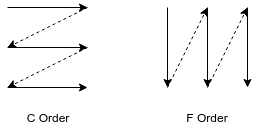
\includegraphics[width=2.5in]{images/c_f_OrdersLabelled.png} 
		\label{fig:cOrders}
	\end{center}
	\[
	A = 
	\begin{bmatrix}
	a_{11} &  a_{12} & a_{13} \\
	a_{21} &  a_{22} & a_{23}
	\end{bmatrix}
	\quad\Rightarrow\quad
	\begin{aligned}
	C-Order = 
	\begin{bmatrix}
	a_{11} &  a_{12} & a_{13} & a_{21} &  a_{22} & a_{23}
	\end{bmatrix}
	\\
	F-Order = 
	\begin{bmatrix}
	a_{11} &  a_{21} & a_{12} & a_{22} &  a_{31} & a_{13}
	\end{bmatrix}
	\end{aligned}
	\]
\caption{Comparison between C-order and F-order}
\label{fig:orders}

\end{figure}

The data are accessed via strides which define how to index over contiguous block of data. For each dimension it defines by how many values two consecutive dimensions are separated. In the case of the matrix $A$ defined in figure \ref{fig:orders}, the strides would be $(3, 1)$ in case of C-order and $(1, 3)$ in case of F-order. Strides $(3, 1)$ means that each row is separated by 3 values and each column is separated by 1 value.

\subsection{Data Buffer}
Databuffer is a storage abstraction. This allows for backend optimal storage


\subsection{Information concerning the shape of the array}
..
\section{Hierarchy of Arrays}
..
\section{Important Component of the Arrays}
..
\subsection{Indexes}
..
\subsection{Views}
..
\subsection{Operations}
..